\documentclass[11pt, a4paper]{article}

% --------------------------------------------------------------------------
% packages
% --------------------------------------------------------------------------
\usepackage[T1]{fontenc}
\usepackage[utf8]{inputenc}
\usepackage[english]{babel}
\usepackage{lmodern}
\usepackage{geometry}
\geometry{margin=2.5cm}

\usepackage{amsmath, amssymb}
\usepackage{amsthm}
\usepackage{booktabs}
\usepackage{array}
\usepackage{caption}
\usepackage{float}
\usepackage{graphicx}
\usepackage{xcolor}
\usepackage{listings}
\usepackage{hyperref}
\usepackage{parskip}

% definition box
\newtheoremstyle{defstyle}{6pt}{6pt}{\normalfont}{}{\bfseries}{.}{.5em}{}
\theoremstyle{defstyle}
\newtheorem*{remark}{Remark}

% --------------------------------------------------------------------------
% hyperref configuration
% --------------------------------------------------------------------------
\hypersetup{
    colorlinks = true,
    linkcolor  = black,
    urlcolor   = blue!60!black,
    citecolor  = black,
    pdftitle   = {FX Option Backtester --- User Guide},
    pdfauthor  = {},
}

% --------------------------------------------------------------------------
% listings configuration (Python and bash)
% --------------------------------------------------------------------------
\definecolor{codebg}{RGB}{245,245,245}
\definecolor{codecomment}{RGB}{100,100,100}
\definecolor{codestring}{RGB}{0,100,0}
\definecolor{codekeyword}{RGB}{0,0,180}

\lstdefinestyle{python}{
    language        = Python,
    backgroundcolor = \color{codebg},
    basicstyle      = \ttfamily\small,
    keywordstyle    = \color{codekeyword}\bfseries,
    stringstyle     = \color{codestring},
    commentstyle    = \color{codecomment}\itshape,
    numbers         = none,
    frame           = single,
    framerule       = 0.4pt,
    breaklines      = true,
    tabsize         = 4,
    showstringspaces= false,
}

\lstdefinestyle{bash}{
    language        = bash,
    backgroundcolor = \color{codebg},
    basicstyle      = \ttfamily\small,
    keywordstyle    = \color{codekeyword}\bfseries,
    commentstyle    = \color{codecomment}\itshape,
    numbers         = none,
    frame           = single,
    framerule       = 0.4pt,
    breaklines      = true,
    showstringspaces= false,
}

% inline code
\newcommand{\code}[1]{\texttt{#1}}

% --------------------------------------------------------------------------
% title
% --------------------------------------------------------------------------
\title{%
    \Large\bfseries FX Option Backtester\\[0.4em]
    \large User Guide
}
\author{}
\date{\today}

% ==========================================================================
\begin{document}
% ==========================================================================

\maketitle

\begin{abstract}
\noindent
This document specifies the design, methodology and quantitative behaviour of a
modular FX option backtester applied to the EUR/NOK currency pair.
Pricing relies on the Garman--Kohlhagen (1983) two-rate extension of Black--Scholes;
risk is managed through a daily delta hedge of the option book against a spot
position, and daily profit and loss is decomposed by Greek via a second-order
Taylor expansion.
The text covers the pricing model, data conventions, interpolation schemes,
strategy life-cycle, hedge accounting, performance and risk metrics, and an
empirical study of the delta-hedged long straddle over 2021--2024.
\end{abstract}

\tableofcontents
\bigskip

\hrule
\vspace{1em}

% ==========================================================================
\section*{Notation}
\addcontentsline{toc}{section}{Notation}
% ==========================================================================

\begin{table}[H]
\centering
\renewcommand{\arraystretch}{1.25}
\begin{tabular}{@{} l l @{}}
    \toprule
    \textbf{Symbol} & \textbf{Definition} \\
    \midrule
    $S_t$       & spot exchange rate (NOK per EUR) at time $t$ \\
    $K$         & strike of the option \\
    $T$         & time to maturity in years (act/365.25) \\
    $r_d$       & continuously-compounded domestic (NOK) interest rate \\
    $r_f$       & continuously-compounded foreign (EUR) interest rate \\
    $\sigma$    & implied volatility (decimal, annualised) \\
    $N(\cdot)$  & standard normal cumulative distribution function \\
    $\phi(\cdot)$ & standard normal probability density function \\
    $C,\,P$     & call and put prices in the domestic currency \\
    $\Delta,\,\Gamma,\,\nu,\,\Theta,\,\rho_d,\,\rho_f$ & first-order Greeks of the option \\
    $F_t^{T}$   & forward outright rate at $t$ for delivery at $T$ \\
    \bottomrule
\end{tabular}
\caption{Notation used throughout the document}
\end{table}

\hrule
\vspace{1em}

% ==========================================================================
\section{Methodology}
% ==========================================================================

% --------------------------------------------------------------------------
\subsection{Pricing --- Garman--Kohlhagen}
% --------------------------------------------------------------------------

Under the domestic risk-neutral measure $\mathbb{Q}_d$, the spot rate follows
the two-rate geometric Brownian motion of Garman and Kohlhagen (1983),

\begin{equation}
    \frac{dS_t}{S_t}
    \;=\;
    (r_d - r_f)\,dt + \sigma\,dW_t^{\mathbb{Q}_d}
\end{equation}

where the drift carries the cost of carry $r_d - r_f$ that reflects the rate
differential between the domestic and foreign yield curves.
FX options are priced in the \textbf{domestic (quote) currency};
for EUR/NOK the quote currency is NOK, so all premia, P\&L and Greeks
are expressed in NOK.

The closed-form solution for European call and put prices reads

\begin{align}
    C &= S_0\,e^{-r_f T}\,N(d_1) - K\,e^{-r_d T}\,N(d_2) \\[4pt]
    P &= K\,e^{-r_d T}\,N(-d_2) - S_0\,e^{-r_f T}\,N(-d_1)
\end{align}

\begin{equation}
    d_1 = \frac{\ln(S_0/K) + (r_d - r_f + \tfrac{1}{2}\sigma^2)\,T}{\sigma\sqrt{T}},
    \qquad
    d_2 = d_1 - \sigma\sqrt{T}
\end{equation}

The full set of first-order Greeks delivered by the pricer is summarised below.

\begin{table}[H]
\centering
\renewcommand{\arraystretch}{1.6}
\begin{tabular}{@{} l l l @{}}
    \toprule
    \textbf{Greek}    & \textbf{Call}                                                       & \textbf{Put} \\
    \midrule
    $\Delta$          & $e^{-r_f T}\,N(d_1)$                                                 & $-e^{-r_f T}\,N(-d_1)$ \\
    $\Gamma$          & \multicolumn{2}{l}{$\dfrac{e^{-r_f T}\,\phi(d_1)}{S_0\,\sigma\sqrt{T}}$} \\
    $\nu$ (vega)      & \multicolumn{2}{l}{$S_0\,e^{-r_f T}\,\phi(d_1)\,\sqrt{T}$} \\
    $\Theta$          & $-\dfrac{S_0\,e^{-r_f T}\,\phi(d_1)\,\sigma}{2\sqrt{T}} - r_d K e^{-r_d T} N(d_2) + r_f S_0 e^{-r_f T} N(d_1)$
                      & $-\dfrac{S_0\,e^{-r_f T}\,\phi(d_1)\,\sigma}{2\sqrt{T}} + r_d K e^{-r_d T} N(-d_2) - r_f S_0 e^{-r_f T} N(-d_1)$ \\
    $\rho_d$          & $K T e^{-r_d T} N(d_2)$                                              & $-K T e^{-r_d T} N(-d_2)$ \\
    $\rho_f$          & $-S_0 T e^{-r_f T} N(d_1)$                                           & $S_0 T e^{-r_f T} N(-d_1)$ \\
    \bottomrule
\end{tabular}
\caption{Closed-form Garman--Kohlhagen Greeks}
\end{table}

\begin{remark}
In the implementation, vega is rescaled to a 1\% absolute vol move
($\nu/100$) and theta is reported per calendar day ($\Theta/365$), to match
trading-desk conventions and the units used in the attribution.
\end{remark}

% --------------------------------------------------------------------------
\subsection{Market data and units}
% --------------------------------------------------------------------------

\begin{table}[h]
\centering
\renewcommand{\arraystretch}{1.3}
\begin{tabular}{@{} l l l @{}}
    \toprule
    \textbf{Dataset}  & \textbf{File pattern}          & \textbf{Unit normalisation} \\
    \midrule
    Spot              & \code{*spot*.parquet}              & NOK per EUR, used as-is \\
    Forward points    & \code{*forwardcurve*.parquet}      & pips $\div$ 10\,000; outright = spot + points \\
    Deposit curves    & \code{*depocurve*.parquet}         & \% $\to$ decimal; NOK = domestic, EUR = foreign \\
    Vol surface       & \code{*volatilitysurface*.parquet} & \% $\to$ decimal \\
    \bottomrule
\end{tabular}
\caption{Market data sources and normalisation conventions}
\end{table}

Stacked frames are \textbf{pivoted once} into \code{\{date: sub-frame\}} maps so the
day-by-day loop avoids repeated boolean masks.

% --------------------------------------------------------------------------
\subsection{Interpolation and extrapolation}
% --------------------------------------------------------------------------

\begin{table}[h]
\centering
\renewcommand{\arraystretch}{1.3}
\begin{tabular}{@{} l l l @{}}
    \toprule
    \textbf{Object}            & \textbf{Interpolation} & \textbf{Extrapolation} \\
    \midrule
    Vol surface (strike)       & cubic spline           & linear, boundary-slope extension, floored $> 0$ \\
    Vol surface (time)         & linear                 & linear \\
    Forward and rate curves    & linear                 & linear; duplicate tenors collapsed \\
    \bottomrule
\end{tabular}
\caption{Interpolation and extrapolation scheme by object}
\end{table}

% --------------------------------------------------------------------------
\subsection{Strategy life-cycle}
% --------------------------------------------------------------------------

\begin{enumerate}
    \item \textbf{Roll scheduler} generates rebalancing dates
          (\code{W-FRI}, \code{MS}, \code{QS}, \ldots).
    \item On each roll date every \textbf{leg} is opened: its strike is resolved from
          the target delta (ATM maps to the forward outright; otherwise the GK delta is
          inverted on a dense strike grid).
    \item The \textbf{sizing designer} (\code{Strategy.size}) converts the target notional
          into a per-leg traded notional (default: scale by the leg ratio).
    \item Positions are \textbf{settled at intrinsic value} on expiry.
\end{enumerate}

% --------------------------------------------------------------------------
\subsection{Daily delta hedging}
% --------------------------------------------------------------------------

Every business day the engine computes the \textbf{net option delta} (in
foreign-currency units) and holds the opposite amount as a spot position.
The hedge is rolled at the prevailing spot; its realised P\&L is booked daily.
Total daily P\&L is therefore:

\begin{equation}
    \mathrm{PnL}_{\mathrm{day}}
    =
    \underbrace{\Delta\,\mathrm{MTM}_{\mathrm{options}}}_{\text{option leg}}
    +
    \underbrace{\text{hedge PnL}}_{\text{spot leg}}
\end{equation}

% --------------------------------------------------------------------------
\subsection{Performance and risk analytics}
% --------------------------------------------------------------------------

Let $\{r_t\}_{t=1}^{T}$ denote the daily strategy P\&L series
(annualisation factor $A = 252$).
The engine reports the following option-aware metrics.

\begin{align}
    \text{Sharpe ratio}    &= \sqrt{A}\,\frac{\bar{r} - r_f / A}{\hat{\sigma}(r)} \\
    \text{Sortino ratio}   &= \sqrt{A}\,\frac{\bar{r} - r_f / A}{\hat{\sigma}_{\!-}(r)},
        \quad \hat{\sigma}_{\!-}(r) = \sqrt{\tfrac{1}{T}\!\sum_t (\min(r_t, 0))^2} \\
    \text{VaR}_{1-\alpha}  &= -\inf\{x : \mathbb{P}(r_t \le x) \ge \alpha\} \\
    \text{CVaR}_{1-\alpha} &= -\mathbb{E}\!\left[\,r_t \,\big|\, r_t \le -\text{VaR}_{1-\alpha}\right] \\
    \text{Max drawdown}    &= \min_{t} \Big(\,C_t - \max_{s \le t} C_s\Big),
        \quad C_t = \sum_{u \le t} r_u
\end{align}

The default confidence level is $\alpha = 95\%$, and $r_f$ is the risk-free
benchmark (taken as zero in the empirical study below).

% --------------------------------------------------------------------------
\subsection{Greeks P\&L attribution}
% --------------------------------------------------------------------------

The daily option P\&L of legs alive on two consecutive days is decomposed via a
second-order Taylor expansion around the previous day's spot, volatility and time,

\begin{equation}
    \Delta P
    \;\approx\;
    \underbrace{\Delta\,\Delta S}_{\text{delta}}
    + \underbrace{\tfrac{1}{2}\,\Gamma\,(\Delta S)^2}_{\text{gamma}}
    + \underbrace{\nu\,\Delta\sigma}_{\text{vega}}
    + \underbrace{\Theta\,\Delta t}_{\text{theta}}
    + \underbrace{\varepsilon}_{\text{residual}}
\end{equation}

The residual $\varepsilon$ collects higher-order cross-Greeks (vanna $\partial
\Delta / \partial \sigma$, volga $\partial \nu / \partial \sigma$),
discretisation error and small inconsistencies in the volatility surface.
Computing the decomposition \textbf{position-by-position over continuing legs}
keeps premium cash flows on rolls out of the decomposition.
The reported delta component is \textbf{net of the hedge P\&L}: a perfect
daily hedge in a frictionless setting drives this leg to zero, so it acts as a
clean diagnostic of hedge slippage.

% --------------------------------------------------------------------------
\subsection{Signals}
% --------------------------------------------------------------------------

A signal maps the spot price history up to a roll date $t$ onto a boolean
(\emph{trade} / \emph{skip}). Two built-in filters are provided.

\paragraph{Momentum filter.}
With look-back $L$, the entry is allowed when the current spot exceeds its simple
moving average,
\begin{equation*}
    \text{trade}_t \;\Leftrightarrow\; S_t \;\ge\; \frac{1}{L}\sum_{i=1}^{L} S_{t-i+1}
\end{equation*}

\paragraph{Realised-volatility filter.}
With look-back $L$ and threshold $\bar{\sigma}$, the entry is allowed when the
annualised realised volatility exceeds the threshold,
\begin{equation*}
    \text{trade}_t \;\Leftrightarrow\;
    \sqrt{A}\,\hat{\sigma}\bigl(\{r_{t-L+1}, \ldots, r_t\}\bigr)
    \;\ge\;
    \bar{\sigma}
\end{equation*}

Filters compose by logical conjunction and are attached to any strategy via the
\code{signal\_fn} constructor argument.

% ==========================================================================
\section{Architecture}
% ==========================================================================

\begin{figure}[h]
    \centering
    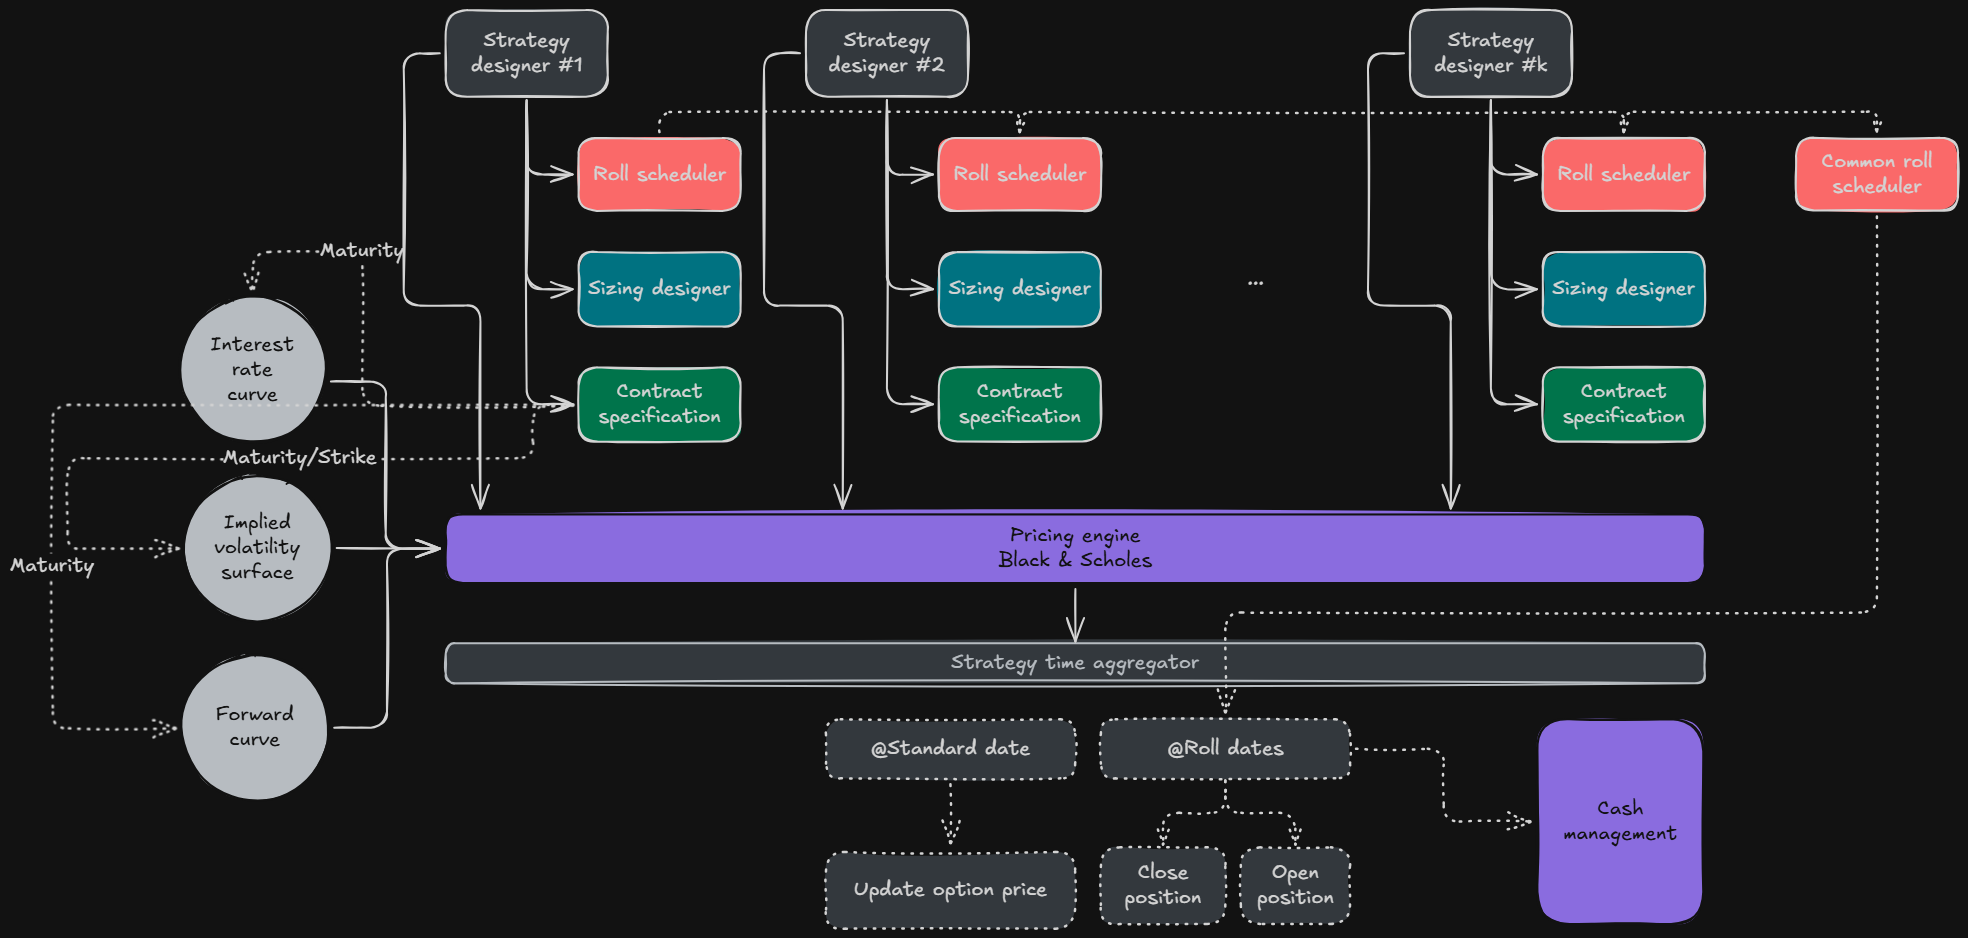
\includegraphics[width=0.92\textwidth]{architecture.png}
    \caption{Component architecture of the FX option backtester}
\end{figure}

\begin{lstlisting}[style=bash, caption={Package layout}]
src/
  data/loader.py          ingest + unit-normalise + pivot stacked Parquet
  curves/interpolator.py  linear curve interpolation/extrapolation
  volatility/surface.py   cubic-spline (strike) / linear (time) vol surface
  pricing/                Garman-Kohlhagen price + Greeks (scalar and vectorised)
  strategies/             Straddle, CallRatioSpread, CalendarSpread, signals, sizing
  portfolio/position.py   option positions, cash, spot delta-hedge book
  analytics/              performance metrics + Greeks P&L attribution
  engine.py               orchestrator: roll -> price -> hedge -> MTM -> attribute
notebooks/backtester.ipynb   end-to-end walkthrough
outputs/                     charts and CSV results (generated by notebook)
\end{lstlisting}

Per-strategy \textbf{roll scheduler}, \textbf{sizing designer} and
\textbf{contract specification} feed a shared Garman--Kohlhagen pricing engine,
whose output is consumed by a time aggregator producing standard-date MTM updates
and roll-date open/close events with cash management.

% ==========================================================================
\section{How to use}
% ==========================================================================

% --------------------------------------------------------------------------
\subsection{Installation}
% --------------------------------------------------------------------------

\begin{lstlisting}[style=bash]
poetry install
# or without Poetry:
pip install pandas numpy scipy matplotlib seaborn pyarrow jupyter
\end{lstlisting}

Place the four Parquet market data files in \code{data/}.

% --------------------------------------------------------------------------
\subsection{Run a backtest}
% --------------------------------------------------------------------------

\begin{lstlisting}[style=python]
from src.engine import Backtester
from src.strategies.straddle import Straddle

bt = Backtester("data")
bt.load_data()

strategy = Straddle(tenor_days=30, direction=1)
results = bt.run(
    strategy,
    start="2021-01-01",
    end="2024-12-31",
    notional=1_000_000,
    roll_freq="W-FRI",
)

print(results["metrics"])
results["daily_pnl"].cumsum().plot()
\end{lstlisting}

\noindent
\code{results} keys: \code{metrics}, \code{daily\_pnl}, \code{components}
(option vs.\ hedge P\&L), \code{greeks}, \code{attribution}, \code{portfolio}.

% --------------------------------------------------------------------------
\subsection{Add a signal}
% --------------------------------------------------------------------------

\begin{lstlisting}[style=python]
from src.strategies.signals import momentum_signal

strategy = Straddle(
    tenor_days=30,
    signal_fn=lambda h: momentum_signal(h, lookback=20),
)
\end{lstlisting}

% --------------------------------------------------------------------------
\subsection{Notebook and tests}
% --------------------------------------------------------------------------

\begin{itemize}
    \item End-to-end walkthrough: \code{notebooks/backtester.ipynb}
    \item Unit tests: \code{poetry run pytest} \\
          Covers pricing parity, Greek signs, curve and vol interpolation,
          performance and attribution analytics.
\end{itemize}

% ==========================================================================
\section{Quantitative deep dive --- delta-hedged long straddle}
% ==========================================================================

\textbf{Setup.}
Long 30-day ATM straddle on EUR/NOK, rolled weekly, delta-hedged daily,
January 2021 to December 2024, notional 1\,000\,000 NOK.

\medskip
\textbf{Economic rationale.}
Once delta is neutralised, the straddle is a pure bet on
\textbf{realised vs.\ implied volatility}. Its carry is approximately

\begin{equation}
    \mathrm{PnL}
    \;\approx\;
    \tfrac{1}{2}\,\Gamma\,S^2
    \bigl(\sigma_{\mathrm{realised}}^2 - \sigma_{\mathrm{implied}}^2\bigr)\,dt
\end{equation}

The strategy harvests gamma when spot moves exceed the implied volatility paid,
and bleeds theta when they do not.

\medskip
\textbf{Backtest results.}

\begin{table}[h]
\centering
\renewcommand{\arraystretch}{1.3}
\begin{tabular}{@{} l r r @{}}
    \toprule
    \textbf{Metric}       & \textbf{Always-on} & \textbf{Momentum-gated} \\
    \midrule
    Total PnL (NOK)       & $\approx 1.30\,\mathrm{M}$  & $\approx 1.68\,\mathrm{M}$ \\
    Sharpe ratio          & 0.13               & 0.23 \\
    Sortino ratio         & 0.15               & 0.24 \\
    Max drawdown          & $\approx -2.87\,\mathrm{M}$ & $\approx -1.61\,\mathrm{M}$ \\
    \bottomrule
\end{tabular}
\caption{Performance comparison: always-on vs.\ momentum-gated straddle}
\end{table}

The \textbf{Greeks attribution} confirms the textbook long-gamma signature:
cumulative gamma $\approx +21\,\mathrm{M}$ is almost entirely offset by theta
$\approx -24\,\mathrm{M}$, with hedged-delta, vega and residual all small.

\begin{figure}[H]
    \centering
    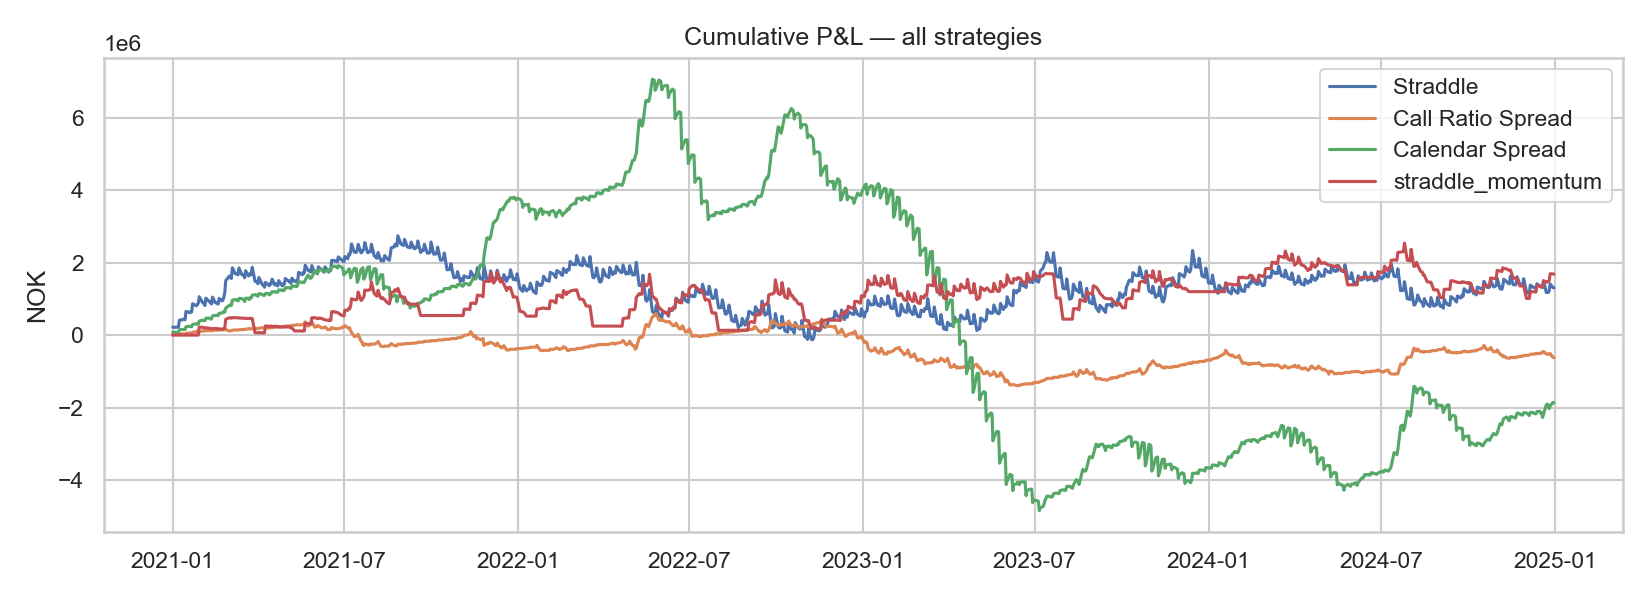
\includegraphics[width=0.95\textwidth]{../outputs/strategy_comparison.png}
    \caption{Cumulative P\&L of the three multi-leg strategies and the momentum-gated
    straddle over the backtest window}
\end{figure}

\medskip
\textbf{Read-through to EUR/NOK.}
NOK is an oil-sensitive, lower-liquidity currency whose volatility clusters in
risk-off episodes (e.g.\ 2022). The gamma harvest dominates during those bursts and
decays in calm, range-bound regimes. A simple momentum filter removes some low-vol
roll periods, roughly \textbf{doubling the Sharpe ratio and halving the maximum
drawdown} while preserving gross P\&L --- a favourable risk-adjusted outcome.

\medskip
\textbf{Limitations.}
Mid-price execution (no bid/ask spread or hedging transaction cost), discrete daily
hedging (gamma slippage between rebalances), and a Taylor attribution that omits
higher-order cross-Greeks (vanna, volga), visible as the residual term.

\medskip
\textbf{Extensions.}
Natural follow-ups include
(i) modelling bid/ask and hedge transaction costs as a haircut on the daily P\&L,
(ii) incorporating stochastic-volatility corrections (vanna/volga adjustment),
(iii) calibrating an intraday rehedging frequency to bound gamma slippage,
(iv) extending the signal library with macroeconomic or risk-on/risk-off filters.

% ==========================================================================
\section*{References}
\addcontentsline{toc}{section}{References}
% ==========================================================================

\begin{itemize}
    \item Garman, M.~B. and Kohlhagen, S.~W. (1983).
          \emph{Foreign currency option values}. Journal of International Money
          and Finance, 2(3), 231--237.
    \item Hull, J.~C. (2018). \emph{Options, Futures, and Other Derivatives},
          10th edition. Pearson.
    \item Reiswich, D. and Wystup, U. (2010).
          \emph{A guide to FX options quoting conventions}. Journal of Derivatives,
          18(2), 58--68.
    \item Wilmott, P. (2007). \emph{Paul Wilmott on Quantitative Finance},
          2nd edition. John Wiley \& Sons.
    \item Bergomi, L. (2016). \emph{Stochastic Volatility Modeling}. Chapman \& Hall.
\end{itemize}

% ==========================================================================
\end{document}
% ==========================================================================
